%%% intro
\begin{frame}{Introdução}

\vspace*{-3em}

O voluntariado é importante porque promove a valorização do meio social e a solidariedade.

\scalebox{0.5}{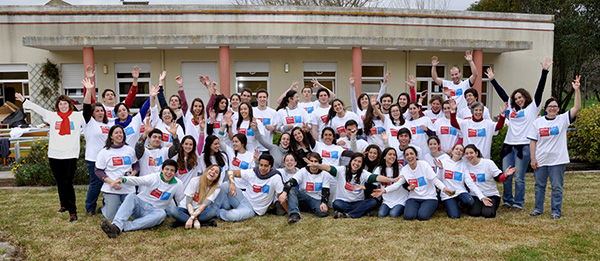
\includegraphics{Figures/volunteering_example}}\\

\vspace*{-1em}
\begin{center}
	{\small Fonte: \url{https://www.unl.pt/}}
\end{center}
\vspace*{-1em}

A participação neste tipo de ações é também uma mais valia para o voluntário devido às \textit{soft skills} adquiridas.

\end{frame}

%%% intro - motivação

\begin{frame}{Introdução - Motivação}

\vspace*{-2em}
\scalebox{0.2}{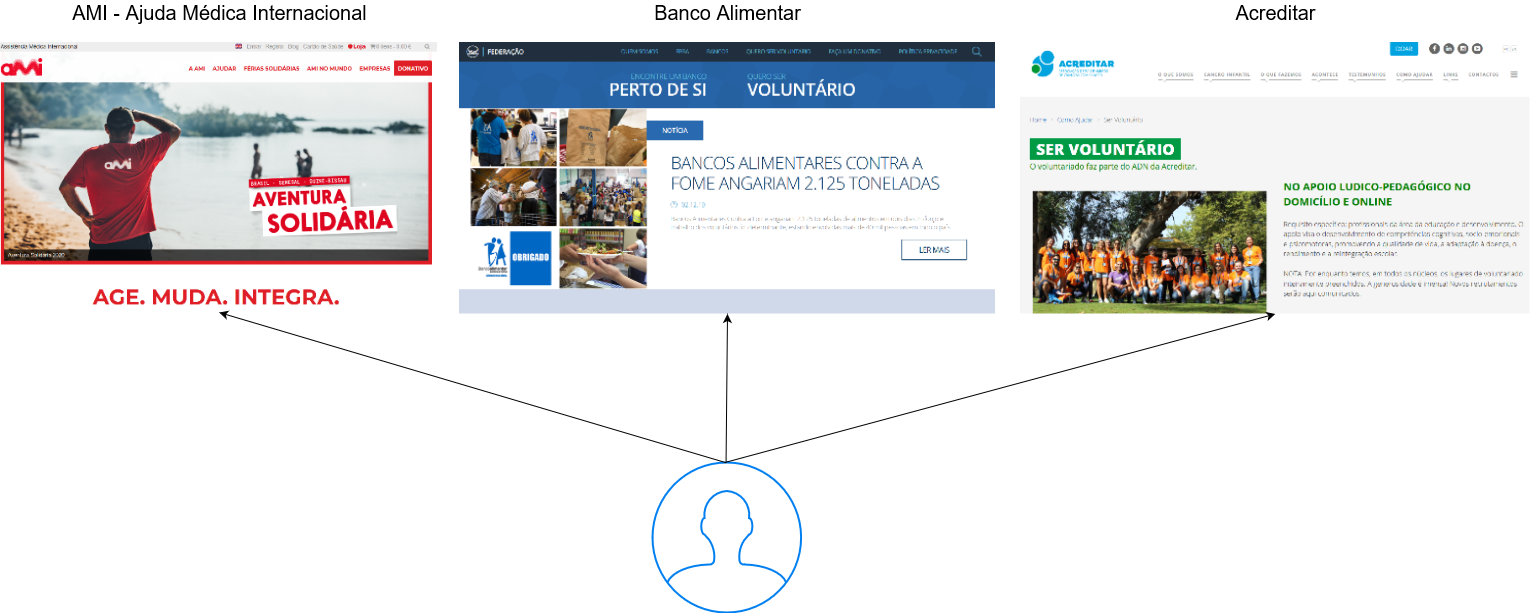
\includegraphics{Figures/services-decentralized}}\\

\vspace*{2em}

{\normalsize As ações de voluntariado são tipicamente divulgadas através de redes sociais ou \textit{websites}. }

\end{frame}

%%% intro - solução

\begin{frame}{Introdução - Solução}

\vspace*{-3em}

Desenvolvimento de uma rede social de voluntariado, onde é possível consultar informações relacionadas com este tipo de ações e interagir com outros utilizadores.

\vspace*{1em}
\scalebox{0.2}{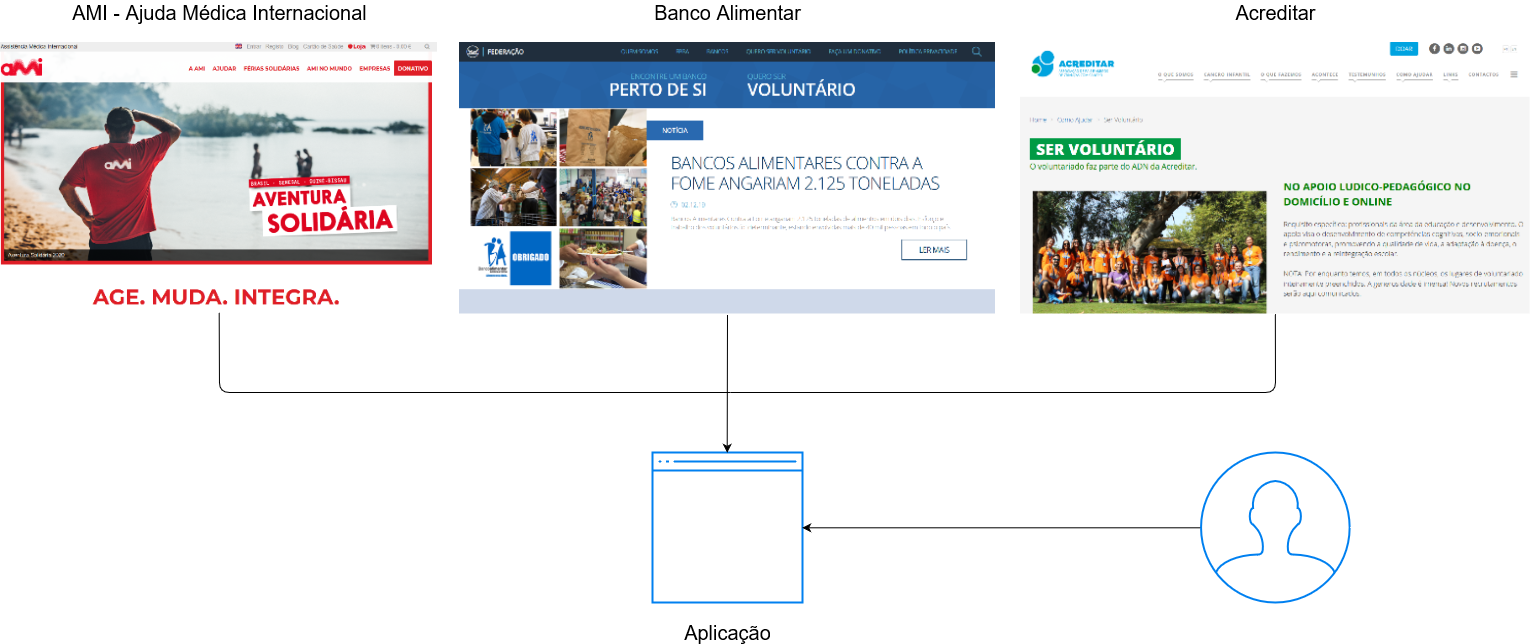
\includegraphics{Figures/services-centralized}}\\

\vspace*{1em}

\end{frame}









